\chapter{The Bean 2 prototype pinout} 
\label{appendix1}
The Bean 2 prototype has 48 pads and was bonded to a 64-lead package from \mbox{Kyocera} Corporation (KYO). The package KYO part number is QC064307WZ. The Bean bonding diagram is shown in Fig.~\ref{fig:bondpad}.
Table~\ref{tab:pinout} shows the Bean V2 pinout.

\begin{center}
\begin{longtable}{|l|l|l|}\hline
{\bf Pin number} & {\bf Pin name} & {\bf Description} \\ \hline\hline
1 & \verb=AGnd= & Analog ground \\\hline
2 & \verb=AGnd= & Analog ground \\\hline
3 & \verb=AGnd= & Analog ground \\\hline
4 & \verb=NC= & No connection \\\hline
5 & \verb=NC= & No connection \\\hline
6 & \verb=res_bias_ext= & IC bias external resistor \\\hline
7 & \verb=V_ref_prechar= & Reference voltage CSA precharger \\\hline
8 & \verb=NC= & No connection  \\\hline
9 &  \verb=clk_prech1= & CSA precharger clk1  \\\hline
10 & \verb=clk_prech2= & CSA precharger clk2  \\\hline
11 & \verb=NC= & No connection \\\hline
12 & \verb=op_mode= & Operation mode select \\\hline
13 & \verb=rst_csa= & CSA reset  \\\hline
14 & \verb=NC= & No connection \\\hline
15 & \verb=cap_precharge_ext= & CSA precharger external capacitor \\\hline
16 & \verb=Vin_csa= & Vin CSA \\\hline
17 & \verb=NC= & No connection \\\hline
18 & \verb=clk= & IC clock \\\hline
19 & \verb=AGnd= & Analog ground \\\hline
20 & \verb=AGnd= & Analog ground \\\hline
21 & \verb=Vi+_fil= & Filter Vi+ \\\hline
{\bf Pin number} & {\bf Pin name} & {\bf Description} \\ \hline\hline
22 & \verb=Vi-_fil= & Filter Vi- \\\hline
23 & \verb=NC= & No connection \\\hline
24 & \verb=Vo-_bp_fil= & Filter bypass Vo- \\\hline
25 & \verb=Vo+_bp_fil= & Filter bypass Vo+  \\\hline
26 & \verb=NC= & No connection \\\hline
27 & \verb=DVdd= & Digital Vdd \\\hline
28 & \verb=DGnd= & Digital Gnd \\\hline
29 & \verb=NC= & No connection \\\hline
30 & \verb=Vo-_fil= & Filter Vo+ (buffered) \\\hline
31 & \verb=Vo+_fil= & Filter Vo- (buffered) \\\hline
32 & \verb=NC= & No connection \\\hline
33 & \verb=out_s= & Filter output selection \\\hline
34 & \verb=Vocm= & Filter Vocm \\\hline
35 & \verb=hold= & Filter hold signal  \\\hline
36 & \verb=rst= & Filter reset \\\hline
37 & \verb=sgn= & Filter gain sign \\\hline
38 & \verb=Vicm= & Filter Vicm \\\hline
39 & \verb=NC= & No connection \\\hline
40 & \verb=AGnd= & Analog ground \\\hline
41 & \verb=NC= & No connection \\\hline
42 & \verb=NC= & No connection \\\hline
43 & \verb=CS_b0= & Filter CS capacitor bit 0 \\\hline
44 & \verb=CS_b1= & Filter CS capacitor bit 1 \\\hline
45 & \verb=CS_b2= & Filter CS capacitor bit 2 \\\hline
46 & \verb=CS_b3= & Filter CS capacitor bit 3 \\\hline
47 & \verb=CS_b4= & Filter CS capacitor bit 4 \\\hline
{\bf Pin number} & {\bf Pin name} & {\bf Description} \\ \hline\hline
48 & \verb=CS_b5= & Filter CS capacitor bit 5 \\\hline
49 & \verb=AGnd= & Analog ground \\\hline
50 & \verb=AGnd= & Analog ground \\\hline
51 & \verb=Vo+_ch= & Channel Vo+ (buffered) \\\hline
52 & \verb=Vo-_ch= & Channel Vo- (buffered)\\\hline
53 & \verb=NC= & No connection \\\hline
54 & \verb=Vout_csa= & CSA Vout (buffered) \\\hline
55 & \verb=NC= & No connection \\\hline
56 & \verb=baseline= & CSA baseline (buffered) \\\hline
57 & \verb=NC= & No connection \\\hline
58 & \verb=NC= & No connection \\\hline
59 & \verb=NC= & No connection \\\hline
60 & \verb=AGnd= & Analog ground \\\hline
61 & \verb=AGnd= & Analog ground \\\hline
62 & \verb=AGnd= & Analog ground \\\hline
63 & \verb=NC= & No connection \\\hline
64 & \verb=AVdd= & Analog Vdd \\\hline
\caption{The Bean 2 prototype pinout}\label{tab:pinout}
\end{longtable}
\end{center}

\begin{figure}[!t]
	\centering
	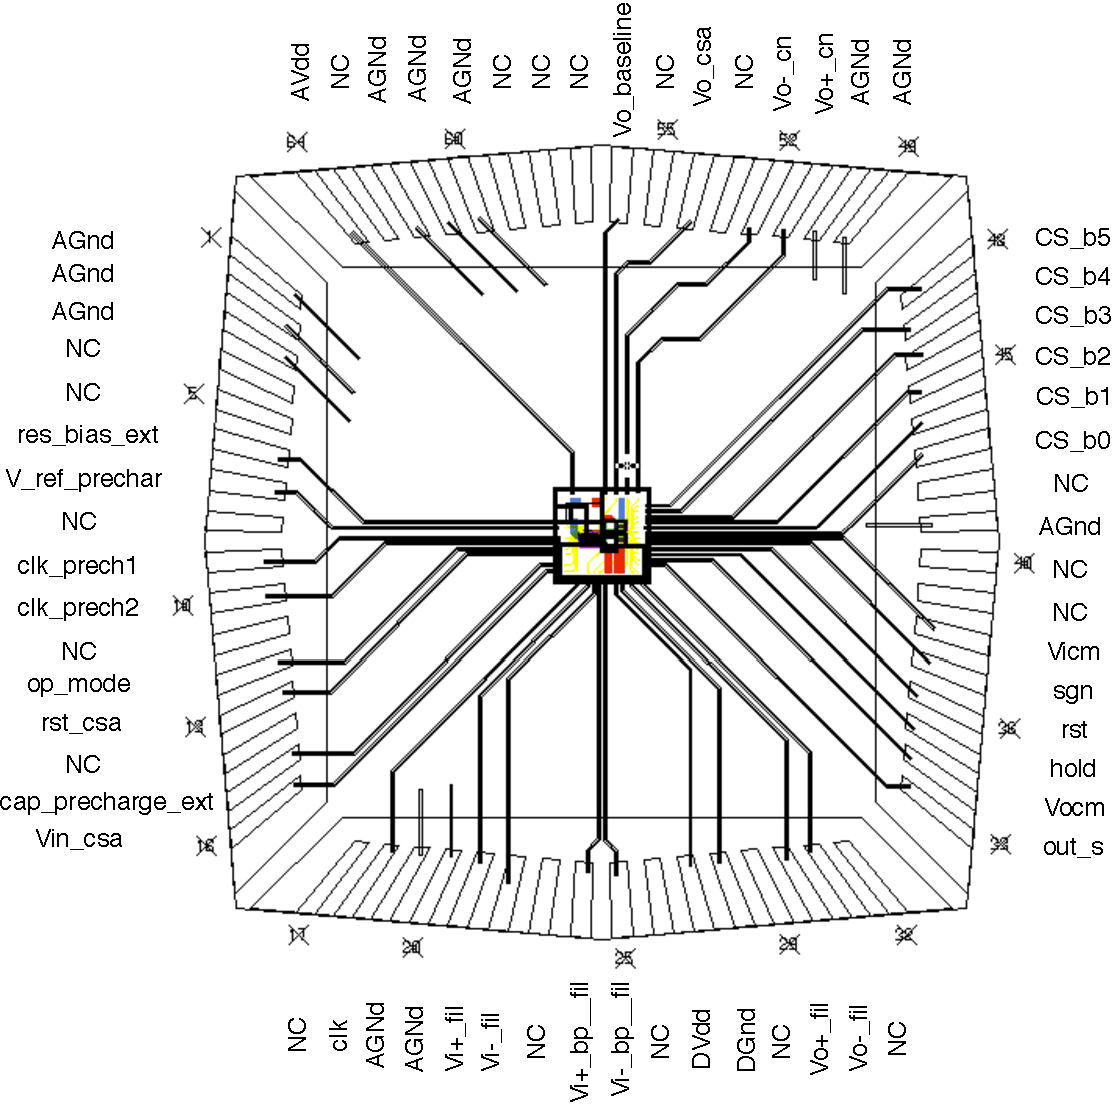
\includegraphics[width=6in]{./Figures/bondpad.pdf}
	\caption{The Bean 2 prototype bonding diagram.}\label{fig:bondpad}
\end{figure}

